\documentclass[]{article}
\usepackage{lmodern}
\usepackage{amssymb,amsmath}
\usepackage{ifxetex,ifluatex}
\usepackage{fixltx2e} % provides \textsubscript
\ifnum 0\ifxetex 1\fi\ifluatex 1\fi=0 % if pdftex
  \usepackage[T1]{fontenc}
  \usepackage[utf8]{inputenc}
\else % if luatex or xelatex
  \ifxetex
    \usepackage{mathspec}
  \else
    \usepackage{fontspec}
  \fi
  \defaultfontfeatures{Ligatures=TeX,Scale=MatchLowercase}
\fi
% use upquote if available, for straight quotes in verbatim environments
\IfFileExists{upquote.sty}{\usepackage{upquote}}{}
% use microtype if available
\IfFileExists{microtype.sty}{%
\usepackage{microtype}
\UseMicrotypeSet[protrusion]{basicmath} % disable protrusion for tt fonts
}{}
\usepackage[margin=1in]{geometry}
\usepackage{hyperref}
\PassOptionsToPackage{usenames,dvipsnames}{color} % color is loaded by hyperref
\hypersetup{unicode=true,
            pdftitle={Lab 03},
            colorlinks=true,
            linkcolor=Maroon,
            citecolor=Blue,
            urlcolor=Blue,
            breaklinks=true}
\urlstyle{same}  % don't use monospace font for urls
\usepackage{color}
\usepackage{fancyvrb}
\newcommand{\VerbBar}{|}
\newcommand{\VERB}{\Verb[commandchars=\\\{\}]}
\DefineVerbatimEnvironment{Highlighting}{Verbatim}{commandchars=\\\{\}}
% Add ',fontsize=\small' for more characters per line
\usepackage{framed}
\definecolor{shadecolor}{RGB}{248,248,248}
\newenvironment{Shaded}{\begin{snugshade}}{\end{snugshade}}
\newcommand{\AlertTok}[1]{\textcolor[rgb]{0.94,0.16,0.16}{#1}}
\newcommand{\AnnotationTok}[1]{\textcolor[rgb]{0.56,0.35,0.01}{\textbf{\textit{#1}}}}
\newcommand{\AttributeTok}[1]{\textcolor[rgb]{0.77,0.63,0.00}{#1}}
\newcommand{\BaseNTok}[1]{\textcolor[rgb]{0.00,0.00,0.81}{#1}}
\newcommand{\BuiltInTok}[1]{#1}
\newcommand{\CharTok}[1]{\textcolor[rgb]{0.31,0.60,0.02}{#1}}
\newcommand{\CommentTok}[1]{\textcolor[rgb]{0.56,0.35,0.01}{\textit{#1}}}
\newcommand{\CommentVarTok}[1]{\textcolor[rgb]{0.56,0.35,0.01}{\textbf{\textit{#1}}}}
\newcommand{\ConstantTok}[1]{\textcolor[rgb]{0.00,0.00,0.00}{#1}}
\newcommand{\ControlFlowTok}[1]{\textcolor[rgb]{0.13,0.29,0.53}{\textbf{#1}}}
\newcommand{\DataTypeTok}[1]{\textcolor[rgb]{0.13,0.29,0.53}{#1}}
\newcommand{\DecValTok}[1]{\textcolor[rgb]{0.00,0.00,0.81}{#1}}
\newcommand{\DocumentationTok}[1]{\textcolor[rgb]{0.56,0.35,0.01}{\textbf{\textit{#1}}}}
\newcommand{\ErrorTok}[1]{\textcolor[rgb]{0.64,0.00,0.00}{\textbf{#1}}}
\newcommand{\ExtensionTok}[1]{#1}
\newcommand{\FloatTok}[1]{\textcolor[rgb]{0.00,0.00,0.81}{#1}}
\newcommand{\FunctionTok}[1]{\textcolor[rgb]{0.00,0.00,0.00}{#1}}
\newcommand{\ImportTok}[1]{#1}
\newcommand{\InformationTok}[1]{\textcolor[rgb]{0.56,0.35,0.01}{\textbf{\textit{#1}}}}
\newcommand{\KeywordTok}[1]{\textcolor[rgb]{0.13,0.29,0.53}{\textbf{#1}}}
\newcommand{\NormalTok}[1]{#1}
\newcommand{\OperatorTok}[1]{\textcolor[rgb]{0.81,0.36,0.00}{\textbf{#1}}}
\newcommand{\OtherTok}[1]{\textcolor[rgb]{0.56,0.35,0.01}{#1}}
\newcommand{\PreprocessorTok}[1]{\textcolor[rgb]{0.56,0.35,0.01}{\textit{#1}}}
\newcommand{\RegionMarkerTok}[1]{#1}
\newcommand{\SpecialCharTok}[1]{\textcolor[rgb]{0.00,0.00,0.00}{#1}}
\newcommand{\SpecialStringTok}[1]{\textcolor[rgb]{0.31,0.60,0.02}{#1}}
\newcommand{\StringTok}[1]{\textcolor[rgb]{0.31,0.60,0.02}{#1}}
\newcommand{\VariableTok}[1]{\textcolor[rgb]{0.00,0.00,0.00}{#1}}
\newcommand{\VerbatimStringTok}[1]{\textcolor[rgb]{0.31,0.60,0.02}{#1}}
\newcommand{\WarningTok}[1]{\textcolor[rgb]{0.56,0.35,0.01}{\textbf{\textit{#1}}}}
\usepackage{graphicx,grffile}
\makeatletter
\def\maxwidth{\ifdim\Gin@nat@width>\linewidth\linewidth\else\Gin@nat@width\fi}
\def\maxheight{\ifdim\Gin@nat@height>\textheight\textheight\else\Gin@nat@height\fi}
\makeatother
% Scale images if necessary, so that they will not overflow the page
% margins by default, and it is still possible to overwrite the defaults
% using explicit options in \includegraphics[width, height, ...]{}
\setkeys{Gin}{width=\maxwidth,height=\maxheight,keepaspectratio}
\IfFileExists{parskip.sty}{%
\usepackage{parskip}
}{% else
\setlength{\parindent}{0pt}
\setlength{\parskip}{6pt plus 2pt minus 1pt}
}
\setlength{\emergencystretch}{3em}  % prevent overfull lines
\providecommand{\tightlist}{%
  \setlength{\itemsep}{0pt}\setlength{\parskip}{0pt}}
\setcounter{secnumdepth}{0}
% Redefines (sub)paragraphs to behave more like sections
\ifx\paragraph\undefined\else
\let\oldparagraph\paragraph
\renewcommand{\paragraph}[1]{\oldparagraph{#1}\mbox{}}
\fi
\ifx\subparagraph\undefined\else
\let\oldsubparagraph\subparagraph
\renewcommand{\subparagraph}[1]{\oldsubparagraph{#1}\mbox{}}
\fi

%%% Use protect on footnotes to avoid problems with footnotes in titles
\let\rmarkdownfootnote\footnote%
\def\footnote{\protect\rmarkdownfootnote}


  \title{Lab 03}
    \author{}
    \date{}
  

% change section title styling
\usepackage{sectsty}
\sectionfont{\normalsize\normalfont\itshape}
\subsectionfont{\normalsize\normalfont}

% use fancyhdr style
\usepackage{fancyhdr}
\pagestyle{fancy}
\fancyhead[LO, LE]{Lab 03}
\fancyhead[RO, RE]{GEOG 491/891}
\makeatletter
\renewcommand{\maketitle}{\bgroup\vspace*{-1cm}\setlength{\parindent}{0pt}
\begin{flushleft}
  \@author
  
  \@date
  
\end{flushleft}\egroup
}
\makeatother

\begin{document}
\maketitle

\hypertarget{lab-03-spatial-autocorrelation-globally-and-locally}{%
\section{Lab 03: Spatial autocorrelation, globally and
locally}\label{lab-03-spatial-autocorrelation-globally-and-locally}}

\hypertarget{read-the-instructions-completely-before-starting-the-lab}{%
\subsubsection{Read the instructions COMPLETELY before starting the
lab}\label{read-the-instructions-completely-before-starting-the-lab}}

This lab builds on many of the discussions and exercises from class,
including previous labs.

\hypertarget{attribution}{%
\subsubsection{Attribution}\label{attribution}}

This lab uses some code examples and directions from
\url{https://mgimond.github.io/Spatial/spatial-autocorrelation-in-r.html}

\hypertarget{formatting-your-submission}{%
\subsubsection{Formatting your
submission}\label{formatting-your-submission}}

This lab must be placed into a public repository on GitHub
(www.github.com). Before the due date, submit \textbf{on Canvas} a link
to the repository. I will then download your repositories and run your
code. The code must be contained in either a .R script or a .Rmd
markdown document. As I need to run your code, any data you use in the
lab must be referenced using \textbf{relative path names}. Finally,
answers to questions I pose in this document must also be in the
repository at the time you submit your link to Canvas. They can be in a
separate text file, or if you decide to use an RMarkdown document, you
can answer them directly in the doc.

\hypertarget{data}{%
\subsection{Data}\label{data}}

The data for this lab can be found on the US Census website.

\begin{enumerate}
\def\labelenumi{\arabic{enumi}.}
\item
  First, go here:
  \url{https://www.census.gov/geographies/mapping-files/2010/geo/tiger-data.html}
\item
  Second, scroll to the ``Demographic Profile 1 - ShapeFile Format''
  section
\item
  Click on ``Counties'' to download the county data for all of the US
  (the direct link is also here:
  \url{http://www2.census.gov/geo/tiger/TIGER2010DP1/County_2010Census_DP1.zip})
\end{enumerate}

\hypertarget{introduction}{%
\subsection{Introduction}\label{introduction}}

In this lab, we will be calculating the spatial autocorrelation of
various Census variables across a subset of the US. Please note, the
dataset you downloaded above is larger than the current 100MB limit
GitHub imposes on single files. This means you'll be unable to push that
dataset to GitHub. Accordingly, I \emph{strongly} suggest you subset the
data such that your files are under this limit. This will be vital when
I grade your submissions. If you're not certain how to save a subset of
the file to disk, look at \texttt{?sf::write\_sf} for help. We will also
be using a new package called \texttt{spdep} in this assignment.

We begin by loading the relevant packages and data

\begin{Shaded}
\begin{Highlighting}[]
\FunctionTok{library}\NormalTok{(spdep)}
\end{Highlighting}
\end{Shaded}

\begin{verbatim}
## Loading required package: sp
\end{verbatim}

\begin{verbatim}
## Loading required package: spData
\end{verbatim}

\begin{verbatim}
## To access larger datasets in this package, install the spDataLarge
## package with: `install.packages('spDataLarge',
## repos='https://nowosad.github.io/drat/', type='source')`
\end{verbatim}

\begin{verbatim}
## Loading required package: sf
\end{verbatim}

\begin{verbatim}
## Linking to GEOS 3.8.1, GDAL 3.2.1, PROJ 7.2.1
\end{verbatim}

\begin{Shaded}
\begin{Highlighting}[]
\FunctionTok{library}\NormalTok{(sf)}
\FunctionTok{library}\NormalTok{(tidyverse)}
\end{Highlighting}
\end{Shaded}

\begin{verbatim}
## -- Attaching packages --------------------------------------- tidyverse 1.3.1 --
\end{verbatim}

\begin{verbatim}
## v ggplot2 3.3.5     v purrr   0.3.4
## v tibble  3.1.2     v dplyr   1.0.7
## v tidyr   1.1.3     v stringr 1.4.0
## v readr   1.4.0     v forcats 0.5.1
\end{verbatim}

\begin{verbatim}
## -- Conflicts ------------------------------------------ tidyverse_conflicts() --
## x dplyr::filter() masks stats::filter()
## x dplyr::lag()    masks stats::lag()
\end{verbatim}

\begin{Shaded}
\begin{Highlighting}[]
\FunctionTok{library}\NormalTok{(tmap)}
\end{Highlighting}
\end{Shaded}

Next, we load our data, look at it, then maybe plot it (the plot might
take some time)

\begin{Shaded}
\begin{Highlighting}[]
\NormalTok{d.all }\OtherTok{\textless{}{-}}\NormalTok{ sf}\SpecialCharTok{::}\FunctionTok{read\_sf}\NormalTok{(}\StringTok{"../data/County\_2010Census\_DP1.shp"}\NormalTok{)}
\FunctionTok{glimpse}\NormalTok{(d.all)}
\end{Highlighting}
\end{Shaded}

\begin{verbatim}
## Rows: 3,221
## Columns: 196
## $ GEOID10    <chr> "02013", "02016", "28107", "28101", "28027", "22065", "5154~
## $ NAMELSAD10 <chr> "Aleutians East Borough", "Aleutians West Census Area", "Pa~
## $ FUNCSTAT10 <chr> "A", "S", "A", "A", "A", "A", "F", "F", "F", "F", "A", "A",~
## $ ALAND10    <dbl> 18083148800, 11370762625, 1774515519, 1497282694, 143081823~
## $ AWATER10   <dbl> 20792209033, 25190643524, 51767046, 3879399, 79539470, 6853~
## $ INTPTLAT10 <chr> "+55.2437223", "+51.9594469", "+34.3652052", "+32.4019702",~
## $ INTPTLON10 <chr> "-161.9507485", "+178.3388130", "-089.9630654", "-089.11841~
## $ DP0010001  <int> 3141, 5561, 34707, 21720, 26151, 12093, 43475, 139966, 6650~
## $ DP0010002  <int> 123, 205, 2552, 1528, 2115, 808, 2305, 9964, 413, 1279, 192~
## $ DP0010003  <int> 105, 227, 2485, 1609, 2015, 838, 1665, 6354, 375, 1253, 183~
## $ DP0010004  <int> 88, 226, 2626, 1510, 2156, 820, 1485, 4630, 403, 1294, 1734~
## $ DP0010005  <int> 104, 249, 2733, 1867, 2327, 863, 2702, 4953, 558, 1221, 169~
## $ DP0010006  <int> 249, 334, 2200, 1275, 1905, 850, 10545, 8142, 623, 1810, 17~
## $ DP0010007  <int> 301, 517, 2094, 1218, 1651, 1021, 4981, 17762, 387, 1726, 1~
## $ DP0010008  <int> 213, 455, 2062, 1282, 1493, 904, 3162, 16419, 389, 1540, 18~
## $ DP0010009  <int> 242, 477, 2168, 1400, 1473, 742, 2186, 13569, 344, 1483, 17~
## $ DP0010010  <int> 355, 660, 2163, 1368, 1454, 720, 2238, 11224, 407, 1626, 16~
## $ DP0010011  <int> 431, 627, 2558, 1397, 1705, 879, 2208, 9706, 409, 1744, 164~
## $ DP0010012  <int> 340, 605, 2531, 1475, 1785, 844, 2145, 8987, 427, 1696, 152~
## $ DP0010013  <int> 264, 458, 2203, 1315, 1582, 775, 2100, 8282, 415, 1410, 124~
## $ DP0010014  <int> 171, 328, 1921, 1243, 1304, 595, 1736, 7168, 432, 1395, 991~
## $ DP0010015  <int> 75, 110, 1419, 958, 955, 457, 1224, 4587, 332, 921, 68641, ~
## $ DP0010016  <int> 33, 47, 1139, 754, 761, 307, 896, 2758, 269, 695, 48095, 10~
## $ DP0010017  <int> 25, 17, 803, 612, 617, 262, 726, 1935, 196, 529, 37439, 964~
## $ DP0010018  <int> 15, 14, 564, 486, 428, 227, 614, 1605, 123, 483, 27990, 659~
## $ DP0010019  <int> 7, 5, 486, 423, 425, 181, 557, 1921, 148, 460, 25807, 548, ~
## $ DP0010020  <int> 2093, 3723, 16683, 10412, 12003, 5986, 20754, 67262, 3093, ~
## $ DP0010021  <int> 68, 106, 1333, 742, 1084, 381, 1166, 5094, 200, 661, 98699,~
## $ DP0010022  <int> 55, 113, 1263, 820, 989, 435, 856, 3178, 185, 651, 93807, 1~
## $ DP0010023  <int> 40, 129, 1353, 808, 1094, 422, 748, 2361, 209, 629, 88229, ~
## $ DP0010024  <int> 63, 149, 1398, 948, 1134, 440, 1264, 2535, 253, 646, 86936,~
## $ DP0010025  <int> 187, 233, 1067, 627, 957, 475, 4816, 3691, 300, 962, 87243,~
## $ DP0010026  <int> 208, 375, 987, 538, 708, 546, 2621, 8233, 196, 916, 99270, ~
## $ DP0010027  <int> 144, 319, 941, 615, 612, 514, 1615, 7980, 186, 796, 93937, ~
## $ DP0010028  <int> 182, 344, 1047, 665, 653, 359, 1090, 6782, 163, 752, 88930,~
## $ DP0010029  <int> 251, 464, 998, 672, 633, 318, 1111, 5699, 202, 801, 83056, ~
## $ DP0010030  <int> 299, 432, 1228, 706, 752, 445, 1086, 4957, 200, 865, 82530,~
## $ DP0010031  <int> 223, 420, 1251, 688, 783, 390, 998, 4313, 199, 822, 75445, ~
## $ DP0010032  <int> 174, 299, 1048, 623, 746, 380, 1007, 3710, 178, 681, 59632,~
## $ DP0010033  <int> 104, 222, 917, 593, 636, 267, 793, 3352, 194, 674, 46472, 8~
## $ DP0010034  <int> 46, 70, 635, 459, 395, 219, 522, 2164, 151, 418, 31365, 719~
## $ DP0010035  <int> 18, 34, 523, 333, 307, 142, 367, 1225, 124, 311, 21287, 477~
## $ DP0010036  <int> 14, 8, 338, 262, 247, 110, 294, 809, 73, 223, 15468, 443, 2~
## $ DP0010037  <int> 12, 6, 220, 188, 138, 80, 231, 622, 38, 185, 10681, 286, 17~
## $ DP0010038  <int> 5, 0, 136, 125, 135, 63, 169, 557, 42, 130, 8015, 214, 15, ~
## $ DP0010039  <int> 1048, 1838, 18024, 11308, 14148, 6107, 22721, 72704, 3557, ~
## $ DP0010040  <int> 55, 99, 1219, 786, 1031, 427, 1139, 4870, 213, 618, 94139, ~
## $ DP0010041  <int> 50, 114, 1222, 789, 1026, 403, 809, 3176, 190, 602, 89704, ~
## $ DP0010042  <int> 48, 97, 1273, 702, 1062, 398, 737, 2269, 194, 665, 85174, 1~
## $ DP0010043  <int> 41, 100, 1335, 919, 1193, 423, 1438, 2418, 305, 575, 82257,~
## $ DP0010044  <int> 62, 101, 1133, 648, 948, 375, 5729, 4451, 323, 848, 84338, ~
## $ DP0010045  <int> 93, 142, 1107, 680, 943, 475, 2360, 9529, 191, 810, 98561, ~
## $ DP0010046  <int> 69, 136, 1121, 667, 881, 390, 1547, 8439, 203, 744, 93273, ~
## $ DP0010047  <int> 60, 133, 1121, 735, 820, 383, 1096, 6787, 181, 731, 89206, ~
## $ DP0010048  <int> 104, 196, 1165, 696, 821, 402, 1127, 5525, 205, 825, 81795,~
## $ DP0010049  <int> 132, 195, 1330, 691, 953, 434, 1122, 4749, 209, 879, 82445,~
## $ DP0010050  <int> 117, 185, 1280, 787, 1002, 454, 1147, 4674, 228, 874, 77463~
## $ DP0010051  <int> 90, 159, 1155, 692, 836, 395, 1093, 4572, 237, 729, 64982, ~
## $ DP0010052  <int> 67, 106, 1004, 650, 668, 328, 943, 3816, 238, 721, 52644, 8~
## $ DP0010053  <int> 29, 40, 784, 499, 560, 238, 702, 2423, 181, 503, 37276, 676~
## $ DP0010054  <int> 15, 13, 616, 421, 454, 165, 529, 1533, 145, 384, 26808, 572~
## $ DP0010055  <int> 11, 9, 465, 350, 370, 152, 432, 1126, 123, 306, 21971, 521,~
## $ DP0010056  <int> 3, 8, 344, 298, 290, 147, 383, 983, 85, 298, 17309, 373, 32~
## $ DP0010057  <int> 2, 5, 350, 298, 290, 118, 388, 1364, 106, 330, 17792, 334, ~
## $ DP0020001  <dbl> 42.1, 40.7, 36.5, 37.1, 32.8, 34.6, 27.8, 35.6, 37.6, 39.1,~
## $ DP0020002  <dbl> 42.1, 41.1, 35.0, 35.7, 30.3, 32.5, 27.7, 35.4, 35.5, 37.2,~
## $ DP0020003  <dbl> 42.3, 39.9, 37.9, 38.3, 34.9, 37.1, 28.0, 35.8, 39.5, 40.7,~
## $ DP0030001  <int> 2811, 4853, 26512, 16739, 19438, 9463, 37697, 118159, 5393,~
## $ DP0030002  <int> 1922, 3350, 12464, 7859, 8620, 4659, 17802, 56202, 2459, 90~
## $ DP0030003  <int> 889, 1503, 14048, 8880, 10818, 4804, 19895, 61957, 2934, 94~
## $ DP0040001  <int> 2770, 4746, 25363, 16067, 18487, 9071, 37001, 115996, 5226,~
## $ DP0040002  <int> 1898, 3294, 11858, 7518, 8159, 4465, 17439, 55111, 2385, 87~
## $ DP0040003  <int> 872, 1452, 13505, 8549, 10328, 4606, 19562, 60885, 2841, 91~
## $ DP0050001  <int> 2684, 4600, 23849, 14821, 17077, 8587, 32740, 113243, 4764,~
## $ DP0050002  <int> 1844, 3190, 11095, 6914, 7454, 4200, 15587, 53655, 2197, 83~
## $ DP0050003  <int> 840, 1410, 12754, 7907, 9623, 4387, 17153, 59588, 2567, 882~
## $ DP0060001  <int> 247, 366, 5526, 3926, 3907, 1765, 4979, 16876, 1331, 3856, ~
## $ DP0060002  <int> 149, 235, 2401, 1704, 1576, 774, 2050, 7290, 547, 1644, 113~
## $ DP0060003  <int> 98, 131, 3125, 2222, 2331, 991, 2929, 9586, 784, 2212, 1511~
## $ DP0070001  <int> 155, 193, 4411, 3233, 3186, 1434, 4017, 12806, 1068, 3088, ~
## $ DP0070002  <int> 95, 118, 1852, 1367, 1222, 614, 1583, 5377, 428, 1267, 8681~
## $ DP0070003  <int> 60, 75, 2559, 1866, 1964, 820, 2434, 7429, 640, 1821, 12115~
## $ DP0080001  <int> 3141, 5561, 34707, 21720, 26151, 12093, 43475, 139966, 6650~
## $ DP0080002  <int> 2988, 5250, 34402, 21531, 26019, 11982, 42166, 134741, 6539~
## $ DP0080003  <int> 660, 2004, 17161, 13734, 5989, 4498, 30031, 85186, 6050, 15~
## $ DP0080004  <int> 219, 332, 16875, 6567, 19752, 7381, 8437, 30491, 347, 1071,~
## $ DP0080005  <int> 876, 857, 76, 1092, 23, 24, 116, 589, 73, 111, 17133, 317, ~
## $ DP0080006  <int> 1130, 1606, 68, 52, 123, 27, 2771, 8432, 29, 3432, 119250, ~
## $ DP0080007  <int> 4, 9, 15, 5, 21, 1, 506, 1761, 4, 615, 37659, 39, 1, 0, 16,~
## $ DP0080008  <int> 3, 8, 21, 12, 65, 7, 884, 1304, 9, 497, 12612, 50, 2, 0, 18~
## $ DP0080009  <int> 1041, 1395, 7, 18, 15, 3, 167, 1379, 0, 321, 8873, 48, 0, 1~
## $ DP0080010  <int> 15, 26, 2, 1, 0, 0, 73, 280, 6, 50, 1897, 4, 0, 0, 3, 4, 24~
## $ DP0080011  <int> 2, 17, 7, 5, 2, 2, 403, 1143, 4, 764, 9825, 9, 0, 0, 1, 3, ~
## $ DP0080012  <int> 28, 123, 3, 11, 7, 11, 143, 485, 1, 544, 26276, 18, 2, 0, 7~
## $ DP0080013  <int> 37, 28, 13, 0, 13, 3, 595, 2080, 5, 641, 22108, 99, 0, 0, 1~
## $ DP0080014  <int> 19, 103, 0, 0, 4, 0, 17, 141, 12, 14, 1222, 15, 0, 1, 5, 2,~
## $ DP0080015  <int> 3, 10, 0, 0, 2, 0, 8, 35, 0, 4, 339, 1, 0, 0, 4, 0, 23, 0, ~
## $ DP0080016  <int> 0, 1, 0, 0, 0, 0, 3, 53, 0, 1, 345, 0, 0, 1, 0, 2, 8, 0, 0,~
## $ DP0080017  <int> 5, 70, 0, 0, 2, 0, 1, 19, 5, 0, 154, 0, 0, 0, 0, 0, 6, 0, 0~
## $ DP0080018  <int> 11, 22, 0, 0, 0, 0, 5, 34, 7, 9, 384, 14, 0, 0, 1, 0, 110, ~
## $ DP0080019  <int> 84, 348, 222, 86, 128, 52, 794, 9902, 28, 1323, 367610, 558~
## $ DP0080020  <int> 153, 311, 305, 189, 132, 111, 1309, 5225, 111, 908, 66863, ~
## $ DP0080021  <int> 59, 90, 79, 59, 4, 29, 132, 372, 40, 86, 6773, 136, 3, 6, 7~
## $ DP0080022  <int> 19, 58, 28, 14, 10, 6, 457, 1423, 14, 334, 7454, 43, 0, 2, ~
## $ DP0080023  <int> 1, 5, 98, 66, 39, 29, 394, 1012, 35, 120, 10195, 155, 1, 15~
## $ DP0080024  <int> 25, 27, 16, 14, 12, 3, 84, 1021, 3, 187, 26207, 231, 6, 45,~
## $ DP0090001  <int> 780, 2221, 17403, 13895, 6065, 4576, 31197, 89445, 6148, 16~
## $ DP0090002  <int> 235, 362, 17048, 6660, 19851, 7452, 9010, 32378, 393, 1278,~
## $ DP0090003  <int> 964, 1000, 211, 1181, 54, 84, 379, 1508, 119, 257, 30403, 5~
## $ DP0090004  <int> 1179, 1743, 109, 72, 160, 41, 3330, 10441, 49, 3874, 132393~
## $ DP0090005  <int> 28, 148, 15, 3, 15, 2, 55, 363, 22, 51, 3458, 56, 0, 1, 10,~
## $ DP0090006  <int> 125, 425, 244, 105, 157, 62, 921, 11504, 37, 1589, 402416, ~
## $ DP0100001  <int> 3141, 5561, 34707, 21720, 26151, 12093, 43475, 139966, 6650~
## $ DP0100002  <int> 385, 726, 494, 287, 293, 188, 2223, 22524, 103, 3556, 90594~
## $ DP0100003  <int> 305, 605, 378, 196, 165, 118, 954, 2352, 49, 348, 762168, 9~
## $ DP0100004  <int> 6, 8, 10, 18, 36, 10, 200, 1603, 8, 164, 8883, 73, 0, 4, 62~
## $ DP0100005  <int> 10, 8, 13, 8, 9, 8, 119, 399, 10, 60, 4279, 22, 0, 0, 4, 9,~
## $ DP0100006  <int> 64, 105, 93, 65, 83, 52, 950, 18170, 36, 2984, 130610, 3541~
## $ DP0100007  <int> 2756, 4835, 34213, 21433, 25858, 11905, 41252, 117442, 6547~
## $ DP0110001  <int> 3141, 5561, 34707, 21720, 26151, 12093, 43475, 139966, 6650~
## $ DP0110002  <int> 385, 726, 494, 287, 293, 188, 2223, 22524, 103, 3556, 90594~
## $ DP0110003  <int> 235, 259, 180, 135, 71, 102, 1204, 10308, 68, 1857, 483168,~
## $ DP0110004  <int> 7, 14, 74, 31, 54, 24, 93, 713, 2, 41, 9468, 102, 0, 21, 25~
## $ DP0110005  <int> 7, 16, 6, 20, 3, 1, 51, 262, 2, 49, 9803, 97, 2, 31, 65, 7,~
## $ DP0110006  <int> 17, 31, 7, 1, 9, 1, 13, 81, 0, 29, 1453, 11, 1, 0, 8, 1, 19~
## $ DP0110007  <int> 0, 1, 0, 0, 0, 0, 4, 32, 0, 3, 348, 2, 0, 0, 0, 2, 17, 0, 0~
## $ DP0110008  <int> 83, 343, 208, 77, 121, 44, 705, 9417, 28, 1275, 364264, 550~
## $ DP0110009  <int> 36, 62, 19, 23, 35, 16, 153, 1711, 3, 302, 37436, 409, 6, 5~
## $ DP0110010  <int> 2756, 4835, 34213, 21433, 25858, 11905, 41252, 117442, 6547~
## $ DP0110011  <int> 425, 1745, 16981, 13599, 5918, 4396, 28827, 74878, 5982, 13~
## $ DP0110012  <int> 212, 318, 16801, 6536, 19698, 7357, 8344, 29778, 345, 1030,~
## $ DP0110013  <int> 869, 841, 70, 1072, 20, 23, 65, 327, 71, 62, 7330, 220, 1, ~
## $ DP0110014  <int> 1113, 1575, 61, 51, 114, 26, 2758, 8351, 29, 3403, 117797, ~
## $ DP0110015  <int> 19, 102, 0, 0, 4, 0, 13, 109, 12, 11, 874, 13, 0, 1, 5, 0, ~
## $ DP0110016  <int> 1, 5, 14, 9, 7, 8, 89, 485, 0, 48, 3346, 76, 0, 1, 11, 9, 5~
## $ DP0110017  <int> 117, 249, 286, 166, 97, 95, 1156, 3514, 108, 606, 29427, 31~
## $ DP0120001  <int> 3141, 5561, 34707, 21720, 26151, 12093, 43475, 139966, 6650~
## $ DP0120002  <int> 1415, 3018, 34392, 21120, 25484, 10502, 41037, 138139, 6250~
## $ DP0120003  <int> 553, 1212, 12839, 8214, 9461, 4025, 17778, 68082, 2603, 834~
## $ DP0120004  <int> 235, 508, 5592, 4017, 3004, 1500, 4996, 22819, 1227, 4431, ~
## $ DP0120005  <int> 440, 887, 10790, 6580, 8740, 3378, 7490, 26785, 1732, 5802,~
## $ DP0120006  <int> 335, 729, 7036, 4761, 5812, 2336, 5586, 21259, 1248, 4156, ~
## $ DP0120007  <int> 66, 156, 3765, 1560, 3117, 1132, 1858, 7577, 358, 1483, 229~
## $ DP0120008  <int> 26, 64, 2135, 813, 1718, 644, 716, 1860, 147, 349, 91091, 1~
## $ DP0120009  <int> 5, 6, 262, 146, 197, 59, 181, 831, 45, 265, 21935, 210, 7, ~
## $ DP0120010  <int> 121, 255, 1406, 749, 1162, 467, 8915, 12876, 330, 1981, 133~
## $ DP0120011  <int> 7, 12, 142, 77, 94, 41, 101, 378, 26, 72, 8400, 133, 2, 18,~
## $ DP0120012  <int> 2, 3, 57, 50, 58, 29, 101, 310, 17, 51, 3854, 51, 2, 15, 31~
## $ DP0120013  <int> 68, 109, 774, 404, 651, 296, 1205, 4691, 148, 369, 56766, 8~
## $ DP0120014  <int> 1726, 2543, 315, 600, 667, 1591, 2438, 1827, 400, 521, 3039~
## $ DP0120015  <int> 0, 4, 139, 159, 256, 1544, 228, 974, 74, 313, 20998, 5768, ~
## $ DP0120016  <int> 0, 1, 97, 79, 147, 995, 96, 594, 18, 95, 14078, 5440, 7, 10~
## $ DP0120017  <int> 0, 3, 42, 80, 109, 549, 132, 380, 56, 218, 6920, 328, 23, 2~
## $ DP0120018  <int> 1726, 2539, 176, 441, 411, 47, 2210, 853, 326, 208, 9400, 3~
## $ DP0120019  <int> 1319, 2047, 66, 219, 248, 32, 1071, 481, 139, 123, 5312, 17~
## $ DP0120020  <int> 407, 492, 110, 222, 163, 15, 1139, 372, 187, 85, 4088, 133,~
## $ DP0130001  <int> 553, 1212, 12839, 8214, 9461, 4025, 17778, 68082, 2603, 834~
## $ DP0130002  <int> 363, 711, 9086, 5802, 6393, 2778, 7518, 30978, 1726, 5545, ~
## $ DP0130003  <int> 198, 408, 3706, 2500, 2882, 1208, 3182, 12919, 703, 2358, 2~
## $ DP0130004  <int> 235, 508, 5592, 4017, 3004, 1500, 4996, 22819, 1227, 4431, ~
## $ DP0130005  <int> 114, 277, 1984, 1557, 1079, 523, 1907, 8972, 448, 1899, 184~
## $ DP0130006  <int> 54, 87, 768, 417, 531, 217, 512, 2306, 123, 310, 49205, 725~
## $ DP0130007  <int> 36, 56, 327, 191, 223, 89, 209, 907, 58, 99, 22276, 367, 12~
## $ DP0130008  <int> 74, 116, 2726, 1368, 2858, 1061, 2010, 5853, 376, 804, 1369~
## $ DP0130009  <int> 48, 75, 1395, 752, 1580, 596, 1066, 3040, 197, 360, 77791, ~
## $ DP0130010  <int> 190, 501, 3753, 2412, 3068, 1247, 10260, 37104, 877, 2802, ~
## $ DP0130011  <int> 147, 393, 3306, 2156, 2691, 1099, 6063, 29564, 753, 2002, 2~
## $ DP0130012  <int> 109, 288, 1548, 942, 1166, 508, 2713, 12626, 268, 812, 1115~
## $ DP0130013  <int> 20, 14, 366, 264, 286, 138, 350, 1426, 95, 179, 15817, 401,~
## $ DP0130014  <int> 38, 105, 1758, 1214, 1525, 591, 3350, 16938, 485, 1190, 128~
## $ DP0130015  <int> 13, 22, 895, 684, 749, 289, 969, 3456, 251, 528, 39941, 863~
## $ DP0140001  <int> 214, 437, 4719, 2934, 3661, 1534, 3587, 14048, 797, 2552, 3~
## $ DP0150001  <int> 90, 95, 3370, 2369, 2439, 1047, 2991, 10061, 777, 2085, 155~
## $ DP0160001  <dbl> 2.56, 2.49, 2.68, 2.57, 2.69, 2.61, 2.31, 2.03, 2.40, 2.64,~
## $ DP0170001  <dbl> 3.04, 3.18, 3.22, 3.10, 3.32, 3.16, 2.91, 2.85, 2.92, 3.11,~
## $ DP0180001  <int> 747, 1929, 14697, 9373, 10792, 4804, 19189, 72376, 2936, 86~
## $ DP0180002  <int> 553, 1212, 12839, 8214, 9461, 4025, 17778, 68082, 2603, 834~
## $ DP0180003  <int> 194, 717, 1858, 1159, 1331, 779, 1411, 4294, 333, 333, 8729~
## $ DP0180004  <int> 45, 85, 384, 205, 488, 177, 671, 2200, 127, 115, 54347, 482~
## $ DP0180005  <int> 1, 34, 9, 18, 20, 6, 59, 143, 5, 9, 1668, 21, 1, 8, 18, 4, ~
## $ DP0180006  <int> 0, 45, 173, 89, 112, 22, 205, 449, 74, 79, 10575, 145, 16, ~
## $ DP0180007  <int> 5, 187, 51, 29, 35, 10, 58, 124, 3, 19, 1937, 56, 8, 94, 22~
## $ DP0180008  <int> 111, 92, 488, 121, 280, 232, 164, 826, 51, 30, 3062, 65, 66~
## $ DP0180009  <int> 32, 274, 753, 697, 396, 332, 254, 552, 73, 81, 15708, 1022,~
## $ DP0190001  <dbl> 0.0, 7.2, 1.8, 1.4, 2.1, 0.9, 2.7, 1.5, 4.1, 1.3, 2.3, 1.8,~
## $ DP0200001  <dbl> 14.3, 9.0, 10.2, 10.3, 10.3, 10.2, 6.0, 5.4, 12.5, 4.5, 11.~
## $ DP0210001  <int> 553, 1212, 12839, 8214, 9461, 4025, 17778, 68082, 2603, 834~
## $ DP0210002  <int> 285, 391, 9472, 6442, 5253, 2471, 7315, 29458, 1720, 5923, ~
## $ DP0210003  <int> 268, 821, 3367, 1772, 4208, 1554, 10463, 38624, 883, 2424, ~
## $ DP0220001  <int> 744, 1091, 25169, 16647, 14205, 6180, 16662, 59938, 4152, 1~
## $ DP0220002  <int> 671, 1927, 9223, 4473, 11279, 4322, 24375, 78201, 2098, 646~
## $ DP0230001  <dbl> 2.61, 2.79, 2.66, 2.58, 2.70, 2.50, 2.28, 2.03, 2.41, 2.63,~
## $ DP0230002  <dbl> 2.50, 2.35, 2.74, 2.52, 2.68, 2.78, 2.33, 2.02, 2.38, 2.67,~
## $ Shape_Leng <dbl> 31.2729207, 53.1754722, 1.7335655, 1.5233734, 2.5172100, 3.~
## $ Shape_Area <dbl> 5.487726055, 4.858872694, 0.178973286, 0.143887112, 0.14778~
## $ geometry   <MULTIPOLYGON [°]> MULTIPOLYGON (((-162.6377 5..., MULTIPOLYGON (~
\end{verbatim}

\begin{Shaded}
\begin{Highlighting}[]
\CommentTok{\#tmap::tm\_shape(d.all) + tm\_polygons() \# commented out because }
\CommentTok{\#it\textquotesingle{}s a large dataset that takes a long time to plot}
\end{Highlighting}
\end{Shaded}

Again, the data are too large, so we need to creat a subset we can work
with later. Let's use the GEOID10 to create a dataset with only those
counties in Nebraska. Be sure to check the data type of GEOID.

\begin{Shaded}
\begin{Highlighting}[]
\CommentTok{\# get just nebraska}
\NormalTok{neb }\OtherTok{\textless{}{-}}\NormalTok{ d.all }\SpecialCharTok{\%\textgreater{}\%}\NormalTok{ dplyr}\SpecialCharTok{::}\FunctionTok{filter}\NormalTok{(stringr}\SpecialCharTok{::}\FunctionTok{str\_starts}\NormalTok{(GEOID10, }\StringTok{"31"}\NormalTok{))}

\CommentTok{\# map it to verify}
\NormalTok{tmap}\SpecialCharTok{::}\FunctionTok{tm\_shape}\NormalTok{(neb) }\SpecialCharTok{+} \FunctionTok{tm\_polygons}\NormalTok{()}
\end{Highlighting}
\end{Shaded}

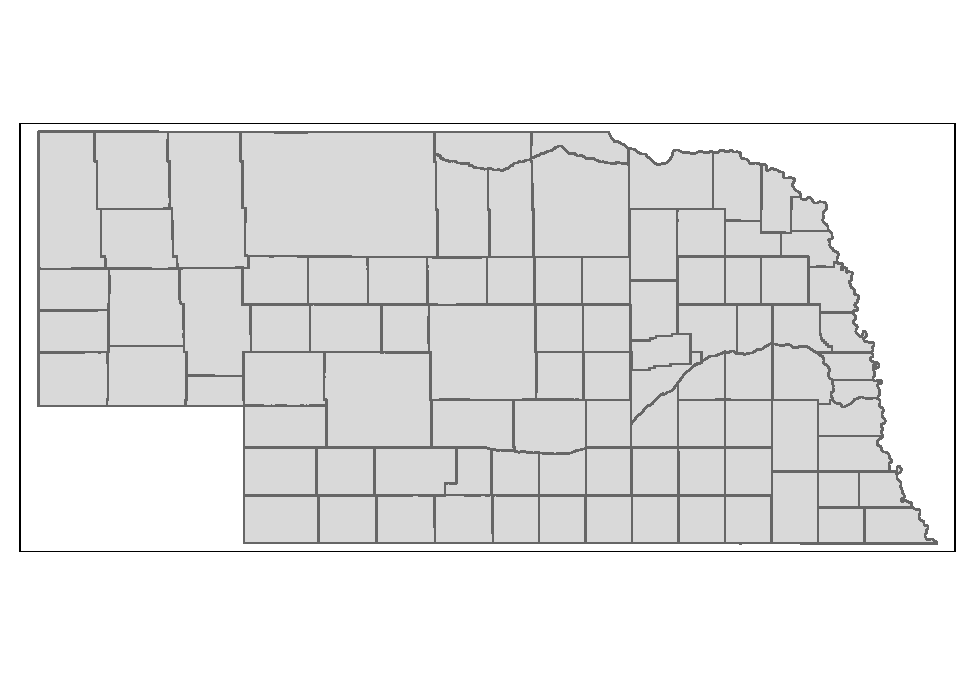
\includegraphics{lab03_files/figure-latex/make_subset-1.pdf}

Next, we'll formalize our space by creating neighbors, and thus,
\textbf{W}

\begin{itemize}
\tightlist
\item
  First we'll project
\item
  Next, we'll use Queen contiguity to define \textbf{W}
\end{itemize}

\begin{Shaded}
\begin{Highlighting}[]
\CommentTok{\# Check it first}
\NormalTok{sf}\SpecialCharTok{::}\FunctionTok{st\_crs}\NormalTok{(neb) }
\end{Highlighting}
\end{Shaded}

\begin{verbatim}
## Coordinate Reference System:
##   User input: NAD83 
##   wkt:
## GEOGCRS["NAD83",
##     DATUM["North American Datum 1983",
##         ELLIPSOID["GRS 1980",6378137,298.257222101,
##             LENGTHUNIT["metre",1]]],
##     PRIMEM["Greenwich",0,
##         ANGLEUNIT["degree",0.0174532925199433]],
##     CS[ellipsoidal,2],
##         AXIS["latitude",north,
##             ORDER[1],
##             ANGLEUNIT["degree",0.0174532925199433]],
##         AXIS["longitude",east,
##             ORDER[2],
##             ANGLEUNIT["degree",0.0174532925199433]],
##     ID["EPSG",4269]]
\end{verbatim}

\begin{Shaded}
\begin{Highlighting}[]
\CommentTok{\# then reproject to north american equidistant conic}
\NormalTok{neb.projected }\OtherTok{\textless{}{-}}\NormalTok{ neb }\SpecialCharTok{\%\textgreater{}\%}\NormalTok{ sf}\SpecialCharTok{::}\FunctionTok{st\_transform}\NormalTok{(., }\StringTok{"ESRI:102010"}\NormalTok{)}

\CommentTok{\# plot it again to make sure nothing broke}
\NormalTok{tmap}\SpecialCharTok{::}\FunctionTok{tm\_shape}\NormalTok{(neb.projected) }\SpecialCharTok{+} \FunctionTok{tm\_polygons}\NormalTok{()}
\end{Highlighting}
\end{Shaded}

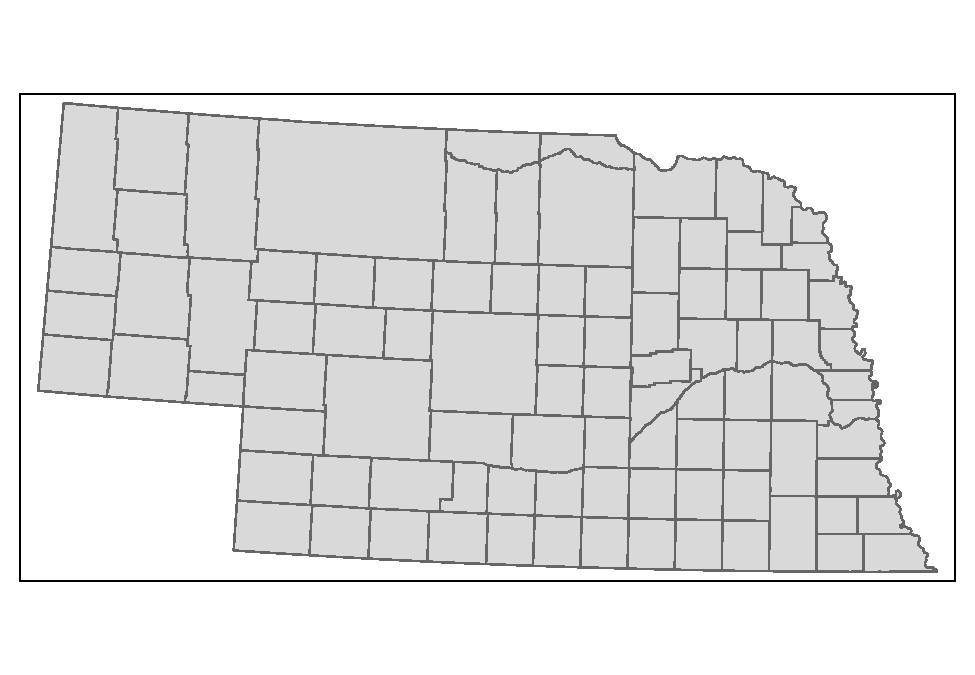
\includegraphics{lab03_files/figure-latex/make some neighbors-1.pdf}

\begin{Shaded}
\begin{Highlighting}[]
\CommentTok{\# make the neighborhood}
\NormalTok{nb }\OtherTok{\textless{}{-}}\NormalTok{ spdep}\SpecialCharTok{::}\FunctionTok{poly2nb}\NormalTok{(neb.projected, }\AttributeTok{queen =} \ConstantTok{TRUE}\NormalTok{)}
\end{Highlighting}
\end{Shaded}

For each polygon in our polygon object, \texttt{nb} lists all
neighboring polygons. For example, to see the neighbors for the first
polygon in the object, type:

\begin{Shaded}
\begin{Highlighting}[]
\NormalTok{nb[[}\DecValTok{1}\NormalTok{]]}
\end{Highlighting}
\end{Shaded}

\begin{verbatim}
## [1] 24 27 43 47
\end{verbatim}

Polygon 1 has 4 neighbors. The numbers represent the polygon IDs as
stored in the spatial object \texttt{neb.projected}. Polygon 1 is
associated with the County attribute name \texttt{"Burt\ County"} and
its four neighboring polygons are associated with the counties:

\begin{Shaded}
\begin{Highlighting}[]
\NormalTok{neb.projected}\SpecialCharTok{$}\NormalTok{NAMELSAD10[}\DecValTok{1}\NormalTok{] }\CommentTok{\# county in index 1}
\end{Highlighting}
\end{Shaded}

\begin{verbatim}
## [1] "Burt County"
\end{verbatim}

\begin{Shaded}
\begin{Highlighting}[]
\NormalTok{nb[[}\DecValTok{1}\NormalTok{]] }\SpecialCharTok{\%\textgreater{}\%}\NormalTok{ neb.projected}\SpecialCharTok{$}\NormalTok{NAMELSAD10[.] }\CommentTok{\# and it\textquotesingle{}s neighbors. }
\end{Highlighting}
\end{Shaded}

\begin{verbatim}
## [1] "Cuming County"     "Thurston County"   "Dodge County"     
## [4] "Washington County"
\end{verbatim}

\begin{Shaded}
\begin{Highlighting}[]
\CommentTok{\# Note we\textquotesingle{}re doing this programmatically step{-}by{-}step}
\end{Highlighting}
\end{Shaded}

Next, we need to assign weights to each neighboring polygon. In our
case, each neighboring polygon will be assigned equal weight
\texttt{(style="W")}. This is accomplished by assigning the fraction:
\texttt{1\ /\ (\ \#\ of\ neighbors)} to each neighboring county then
summing the weighted values. While this is the most intuitive way to
summaries the neighbors' values it has one drawback in that polygons
along the edges of the study area will base their lagged values on fewer
polygons thus potentially over- or under-estimating the true nature of
the spatial autocorrelation in the data. For this example, we'll stick
with the \texttt{style="W"} option for simplicity's sake but note that
other more robust options are available, notably \texttt{style="B"}.

\begin{Shaded}
\begin{Highlighting}[]
\NormalTok{lw }\OtherTok{\textless{}{-}} \FunctionTok{nb2listw}\NormalTok{(nb, }\AttributeTok{style=}\StringTok{"W"}\NormalTok{, }\AttributeTok{zero.policy=}\ConstantTok{TRUE}\NormalTok{)}
\end{Highlighting}
\end{Shaded}

The \texttt{zero.policy=TRUE} option allows for lists of non-neighbors.
This should be used with caution since the user may not be aware of
missing neighbors in their dataset. However, a zero.policy of
\texttt{FALSE} would return an error if you have a dataset where a
polygon does not have a neighbor.

To see the weight of the first polygon's four neighbors type:

\begin{Shaded}
\begin{Highlighting}[]
\NormalTok{lw}\SpecialCharTok{$}\NormalTok{weights[}\DecValTok{1}\NormalTok{]}
\end{Highlighting}
\end{Shaded}

\begin{verbatim}
## [[1]]
## [1] 0.25 0.25 0.25 0.25
\end{verbatim}

This row-normalized our weights!

We can also plot the distribution of neighbors across the dataset.

\begin{Shaded}
\begin{Highlighting}[]
\CommentTok{\# use attr to get the count of neighbors in W}
\NormalTok{neighbors }\OtherTok{\textless{}{-}} \FunctionTok{attr}\NormalTok{(lw}\SpecialCharTok{$}\NormalTok{weights,}\StringTok{"comp"}\NormalTok{)}\SpecialCharTok{$}\NormalTok{d }

\CommentTok{\# plot it}
\FunctionTok{hist}\NormalTok{(neighbors)}
\end{Highlighting}
\end{Shaded}

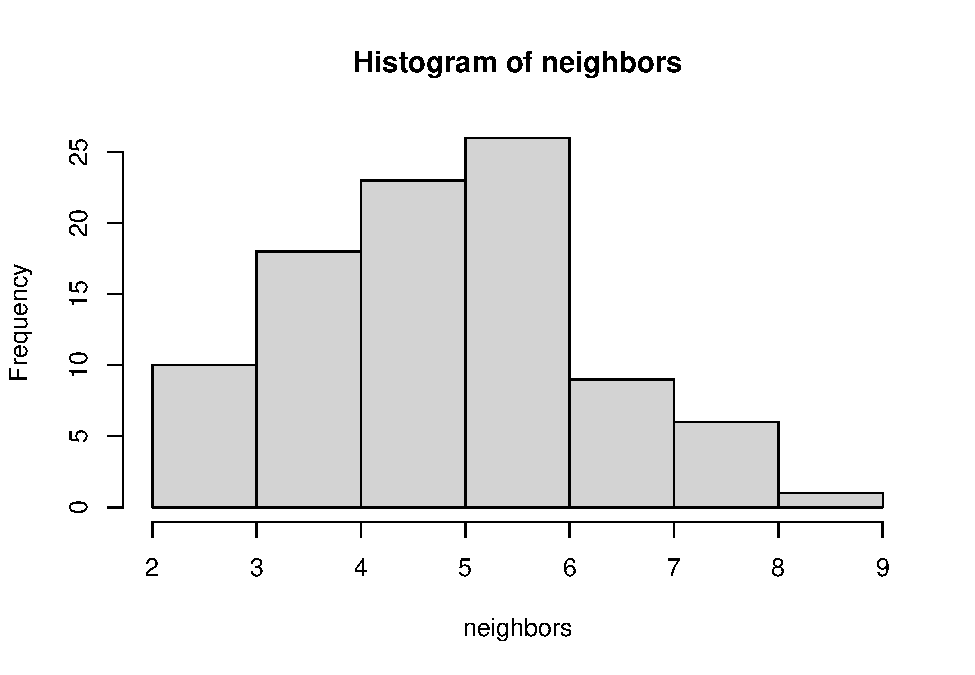
\includegraphics{lab03_files/figure-latex/plotneighbors-1.pdf}

Finally, we'll compute the average neighbor population of Females
\textgreater{} 65 years of age for each polygon. These values are often
referred to as spatially lagged values. The following table shows the
average neighboring F \textgreater65 values (stored in the F65.lag
object) for each county.

\begin{Shaded}
\begin{Highlighting}[]
\NormalTok{F65.lag }\OtherTok{\textless{}{-}} \FunctionTok{lag.listw}\NormalTok{(lw, neb.projected}\SpecialCharTok{$}\NormalTok{DP0070003)}
\NormalTok{F65.lag}
\end{Highlighting}
\end{Shaded}

\begin{verbatim}
##  [1]  1741.7500  1542.6667 10628.1667   185.8000  1135.5000   640.6000
##  [7]  1819.6667   622.2500  1208.5000   670.2500   884.5000   456.0000
## [13]  1386.7500   624.0000  1170.8333  1600.0000   214.8000  1802.2000
## [19]   547.0000   289.2000   566.6667  3766.3333  1050.2857  1203.5000
## [25]   490.0000   701.3333   932.8000  1183.8333   587.0000  3648.5714
## [31]  1199.2000   310.0000  1501.0000   326.8000  1168.4000   641.3333
## [37]  1294.0000  4698.8000   618.1250   176.0000   432.0000   362.2000
## [43]  5543.2857   235.0000 11847.3333   440.0000 12176.6667   458.1667
## [49]  1039.4000  3680.0000  7188.2500   216.4286  1216.0000  4621.4000
## [55]   614.0000  1094.1429   672.2500  1403.3333   890.5000  1595.5000
## [61]   563.4000   932.4000   804.5000   579.0000  1349.0000   428.6667
## [67]   491.5000   960.2500   690.5000  1075.1429  1777.6667  3792.3750
## [73]   817.2000   930.5000  1098.0000  1658.6000   481.6000  1018.8333
## [79]   658.2500  1025.0000   822.8333  3754.0000   901.4286   743.8333
## [85]   992.6000   428.2000  1494.2500  1719.6667   377.1250   948.1250
## [91]  1004.4286  1089.4444  1639.3750
\end{verbatim}

\hypertarget{computing-morans-i}{%
\subsubsection{Computing Moran's I}\label{computing-morans-i}}

To get the Moran's I value, simply use the moran.test function.

\begin{Shaded}
\begin{Highlighting}[]
\FunctionTok{moran.test}\NormalTok{(neb.projected}\SpecialCharTok{$}\NormalTok{DP0070003, lw)}
\end{Highlighting}
\end{Shaded}

\begin{verbatim}
## 
##  Moran I test under randomisation
## 
## data:  neb.projected$DP0070003  
## weights: lw    
## 
## Moran I statistic standard deviate = 3.3554, p-value = 0.0003963
## alternative hypothesis: greater
## sample estimates:
## Moran I statistic       Expectation          Variance 
##       0.138417655      -0.010869565       0.001979517
\end{verbatim}

Note that the p-value computed from the \texttt{moran.test} function is
not computed from an MC simulation but \textbf{analytically} instead.
This may not always prove to be the most accurate measure of
significance. To test for significance using the MC simulation method
instead, use the moran.mc function.

\begin{Shaded}
\begin{Highlighting}[]
\NormalTok{MC}\OtherTok{\textless{}{-}} \FunctionTok{moran.mc}\NormalTok{(neb.projected}\SpecialCharTok{$}\NormalTok{DP0070003, lw, }\AttributeTok{nsim=}\DecValTok{999}\NormalTok{)}

\CommentTok{\# View results (including p{-}value)}
\NormalTok{MC}
\end{Highlighting}
\end{Shaded}

\begin{verbatim}
## 
##  Monte-Carlo simulation of Moran I
## 
## data:  neb.projected$DP0070003 
## weights: lw  
## number of simulations + 1: 1000 
## 
## statistic = 0.13842, observed rank = 977, p-value = 0.023
## alternative hypothesis: greater
\end{verbatim}

\begin{Shaded}
\begin{Highlighting}[]
\CommentTok{\# Plot the distribution}

\CommentTok{\# Plot the distribution (note that this is a density plot instead of a histogram)}
\FunctionTok{plot}\NormalTok{(MC, }\AttributeTok{main=}\StringTok{""}\NormalTok{, }\AttributeTok{las=}\DecValTok{1}\NormalTok{)}
\end{Highlighting}
\end{Shaded}

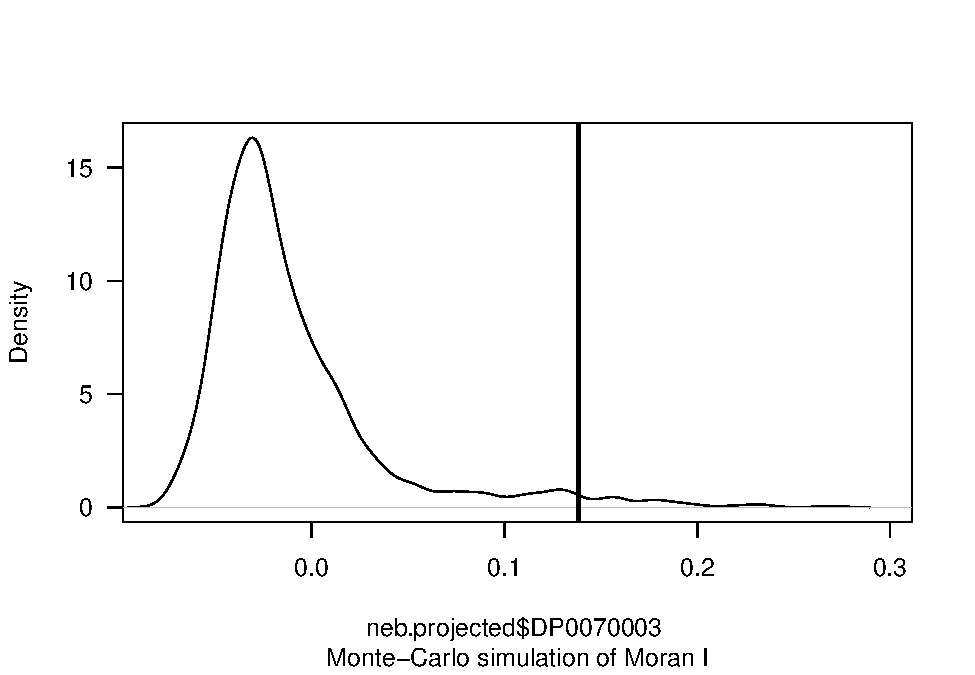
\includegraphics{lab03_files/figure-latex/moranmc-1.pdf}

What is being plotted in this density plot?

\hypertarget{defining-w-using-a-distance-band}{%
\subsubsection{\texorpdfstring{Defining \textbf{W} using a distance
band}{Defining W using a distance band}}\label{defining-w-using-a-distance-band}}

Next, we will explore spatial autocorrelation as a function of distance
bands.

Instead of defining neighbors as contiguous polygons, we will define
neighbors based on distances to \textbf{polygon centers}. We therefore
need to extract the center of each polygon. The object \texttt{coords}
stores all pairs of coordinate values corresponding to polygon
centroids. Note, we need to convert from an \texttt{sf} object to a
\texttt{spatial} one for the \texttt{coordinates()} function to work.

\begin{Shaded}
\begin{Highlighting}[]
\NormalTok{coords }\OtherTok{\textless{}{-}}\NormalTok{ neb.projected }\SpecialCharTok{\%\textgreater{}\%} \FunctionTok{as\_Spatial}\NormalTok{() }\SpecialCharTok{\%\textgreater{}\%} \FunctionTok{coordinates}\NormalTok{()}
\end{Highlighting}
\end{Shaded}

Next, we will define the search radius to include all neighboring
polygon centers within 50 km (or 50,000 meters)

\begin{Shaded}
\begin{Highlighting}[]
\NormalTok{s.dist  }\OtherTok{\textless{}{-}}  \FunctionTok{dnearneigh}\NormalTok{(coords, }\DecValTok{0}\NormalTok{, }\DecValTok{50000}\NormalTok{)}
\end{Highlighting}
\end{Shaded}

The dnearneigh function takes on three parameters:

\begin{enumerate}
\def\labelenumi{\arabic{enumi}.}
\item
  the coordinate values \texttt{coords}
\item
  the radius for the inner radius of the annulus band
\item
  and the radius for the outer annulus band.
\end{enumerate}

In our example, the inner annulus radius is 0 which implies that all
polygon centers up to 50km are considered neighbors.

\textbf{Note that if we chose to restrict the neighbors to all polygon
centers between 50 km and 100 km, for example, then we would define a
search annulus (instead of a circle) as
\texttt{dnearneigh(coords,\ 50000,\ 100000)}}

Now that we defined our search circle, we need to identify all
neighboring polygons for each polygon in the dataset.

\begin{Shaded}
\begin{Highlighting}[]
\NormalTok{lw }\OtherTok{\textless{}{-}} \FunctionTok{nb2listw}\NormalTok{(s.dist, }\AttributeTok{style=}\StringTok{"W"}\NormalTok{,}\AttributeTok{zero.policy=}\NormalTok{T) }

\CommentTok{\#Run the MC simulation.}
\NormalTok{MI  }\OtherTok{\textless{}{-}}  \FunctionTok{moran.mc}\NormalTok{(neb.projected}\SpecialCharTok{$}\NormalTok{DP0070003, lw, }\AttributeTok{nsim=}\DecValTok{999}\NormalTok{, }\AttributeTok{zero.policy=}\NormalTok{T) }

\CommentTok{\#Plot the results.}
\FunctionTok{plot}\NormalTok{(MI, }\AttributeTok{main=}\StringTok{""}\NormalTok{, }\AttributeTok{las=}\DecValTok{1}\NormalTok{) }
\end{Highlighting}
\end{Shaded}

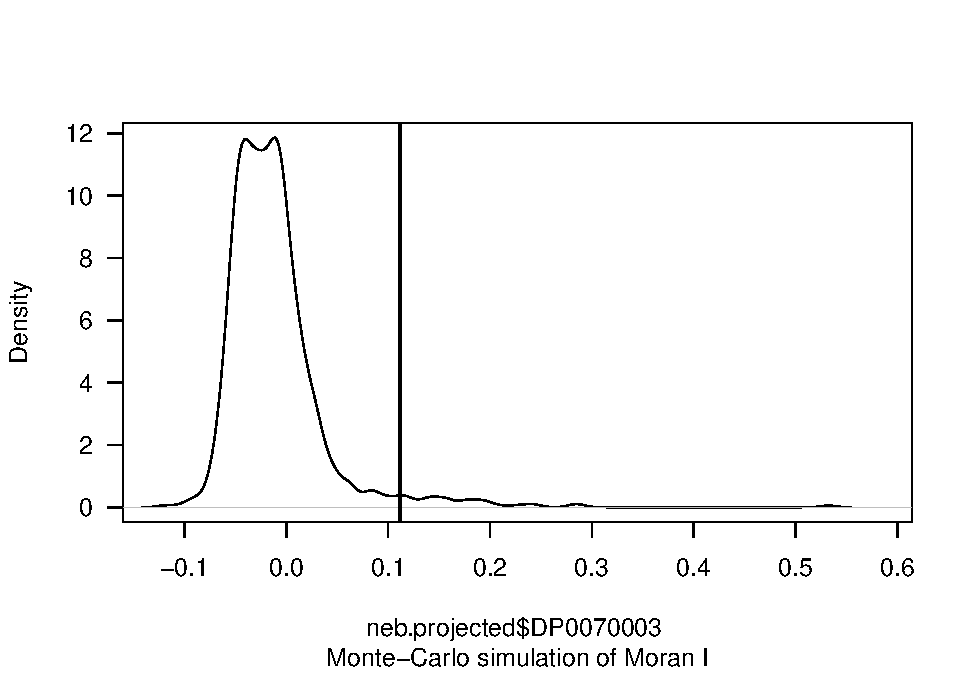
\includegraphics{lab03_files/figure-latex/calcnb-1.pdf}

\begin{Shaded}
\begin{Highlighting}[]
\CommentTok{\#Display p{-}value and other summary statistics.}
\NormalTok{MI}
\end{Highlighting}
\end{Shaded}

\begin{verbatim}
## 
##  Monte-Carlo simulation of Moran I
## 
## data:  neb.projected$DP0070003 
## weights: lw  
## number of simulations + 1: 1000 
## 
## statistic = 0.11161, observed rank = 962, p-value = 0.038
## alternative hypothesis: greater
\end{verbatim}

\hypertarget{morans-plots}{%
\subsubsection{Moran's plots}\label{morans-plots}}

Thus far, our analysis has been a global investigation of spatial
autocorrelation. We can also use local indicators of spatial
autocorrelation (LISA) to analyze our dataset. One way of doing so is
through the use of a Moran plot.

The process to make a plot is relatively simple:

\begin{Shaded}
\begin{Highlighting}[]
\CommentTok{\# use zero.policy = T because some polygons don\textquotesingle{}t have neighbors}
\FunctionTok{moran.plot}\NormalTok{(neb.projected}\SpecialCharTok{$}\NormalTok{DP0070003, lw, }\AttributeTok{zero.policy=}\ConstantTok{TRUE}\NormalTok{, }\AttributeTok{plot=}\ConstantTok{TRUE}\NormalTok{)}
\end{Highlighting}
\end{Shaded}

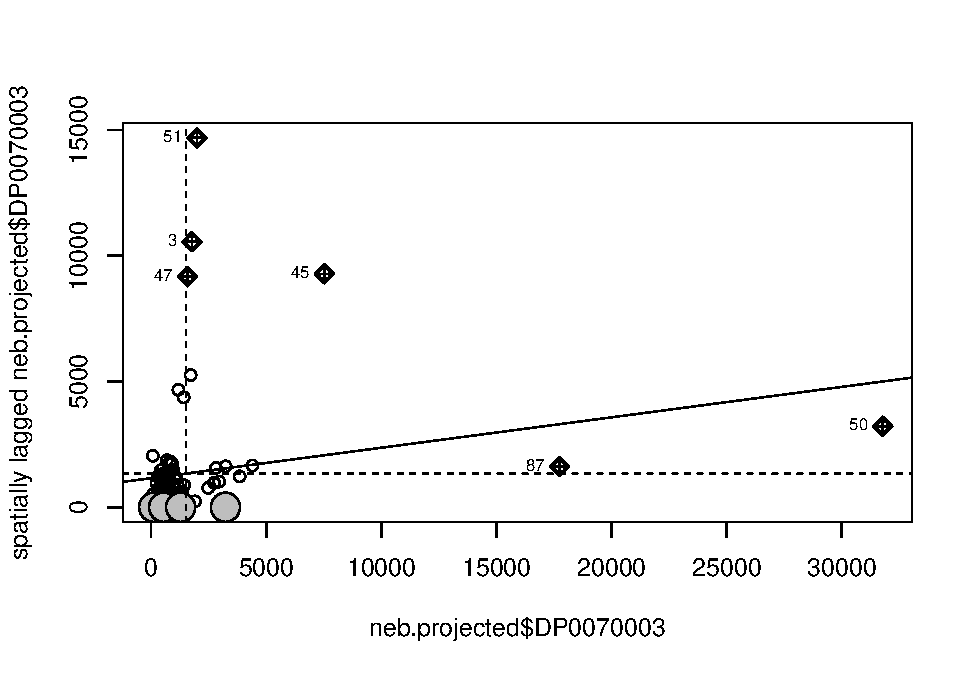
\includegraphics{lab03_files/figure-latex/moranplot-1.pdf}

\hypertarget{your-tasks}{%
\subsection{Your tasks}\label{your-tasks}}

\begin{enumerate}
\def\labelenumi{\arabic{enumi}.}
\item
  Create a spatial subset of the US, with at AT MINIMUM 4 states,
  MAXIMUM 7 states. States must be contiguous. Save this subset as a
  shapefile such that it's sufficiently small in size that GitHub will
  accept the git-push
\item
  Choose a variable. If it's a raw count, you should normalize the
  variable in an appropriate manner (e.g., by total population, percent,
  by area)
\item
  Make a histogram of your chosen variable
\item
  Make a choropleth map of your chosen variable. Choose an appropriate
  data classification scheme
\item
  Develop a contiguity-based spatial weights matrix of your choosing
  (i.e., rook or queen)
\item
  Row-standardize the W
\item
  Plot a histogram of the number of neighbors
\item
  Calculate the average number of neighbors
\item
  Make a Moran Plot
\item
  Repeat \#5 (and 5.1 - 5.4) above with a W developed using the IDW
  method. You will need to investigate the \texttt{spdep} documentation
  to find the correct method/function.
\end{enumerate}

\hypertarget{questions}{%
\subsection{Questions:}\label{questions}}

\begin{enumerate}
\def\labelenumi{\arabic{enumi}.}
\item
  Describe in your own words how Moran's I is calculated
\item
  Describe in your own words: what is a spatially-lagged variable?
\item
  How does your analysis in this lab (as simple as it is) diffr by how
  you have formalized W (e.g., space, neighbors) in two different
  methods? How might it affect analysis?
\item
  What does it mean if an observation falls in the ``H-L'' quadrant? Why
  might it be useful to detect such occurances?
\end{enumerate}

\hypertarget{bonus-50-points}{%
\subsection{Bonus (+50 points)}\label{bonus-50-points}}

B1. make another Moran plot, this time do so manually (use
\texttt{geom\_point} from \texttt{ggplot}). You must label each quadrant
with HH, HL, LL, and LH, respectively. You should also use color and/or
shape to denote whether an observation is statistically significant.
Tip, you can find the data you want using the \texttt{moran.plot}
function, but you'll have to alter the function call and read some
documentation.

B1. plot a choropleth map of your dataset with a categorical color
scheme, where the shading corresponds to the Moran plot (really,
``LISA'') quadrants. Thus, your map will have four shades of color.


\end{document}